We measure the quality factors of the membrane resonator in our setup, by moving to lower wavelengths (roughly \SI{730}{\nano\meter}). At this wavelength our cavity is so transmissive that  cavity enhanced radiation pressure effects can be neglected. We then optically excite the membrane using radiation pressure force. The optical excitation is done by switching to the alternative input (see figure \ref{fig:presetup}) and increasing the input power to roughly \SI{3}{\milli\watt}. The voltage sent to the AOD is modulated by using a TTL switch board. For this we use two signal generators. The first signal generator\footnote{Rohde \& Schwartz SMC100A} modulates the AOD voltage at the mechanical frequency and the second signal generator\footnote{HP 33120A} puts an overall modulation on top of the first signal, which is much slower than the mechanical frequency. Thus the alternative input consists of small bursts of excitation followed by a period where the AOD is not fed any voltage signal so we can detect a signal. For detection we have swapped transmission detector\footnote{Thorlabs PDA8}, because the other detector does not tolerate the high powers we need for excitation. The detector output is sent to a lock-in amplifier\footnote{Zurich Instruments HF2LI} and is here demodulated at the mechanical frequency from the first signal generator. We look for the narrow mechanical resonance by scanning the frequency of the first signal generator. When the mechanical resonance is found we slowly decrease the frequency of the second signal generator to accommodate for the ringdown time, i.e. detecting the actual signal and not interrupting it by yet another excitation burst. The ringdown time trace is then recorded on the oscilloscope. See figure \ref{fig:ringdown_trace} for an example trace.

\begin{figure}[h]
\centering
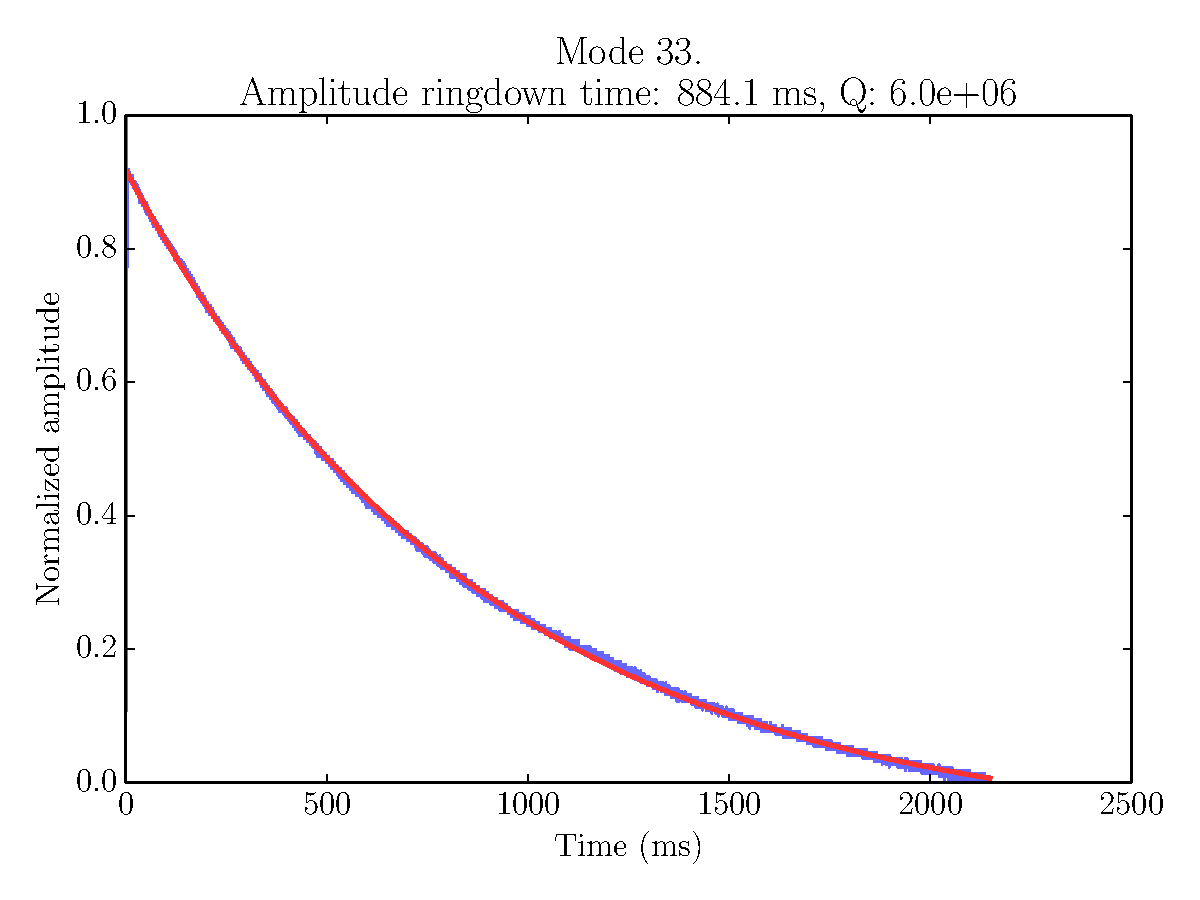
\includegraphics[scale=0.8]{analysis/ringdown_33_4k.pdf}
\caption{Ringdown time trace recorded at cryogenic temperatures.}
\label{fig:ringdown_trace}
\end{figure}

From the eight recorded ringdown traces of the (3,3)-mode at cryogenic temperature we get a quality factor of

\begin{equation}
Q = (6.0 \pm 0.5) \times 10^6,
\end{equation}
\noindent
where the uncertainty is the standard deviation of the measured values. We confirm that the quality factor of the mechanical mode is in fact high and therefore a good prospect for optomechanical induced cooling experiments. The mechanical damping rate is $\Gamma_m/2\pi \approx $ \SI{0.4}{\hertz}.

The use of a secondary signal generator could have been avoided by using a secondary laser beam to detect the signal. Our procedure makes things more complicated and tedious. Because the mechanical resonance is jumping around on the scale of a few \SI{}{\hertz}, while the linewidth is often also \SI{}{\hertz} scale. This makes tracking the resonance and adjusting the timescales a bit difficult.